\chapter{Implementation of the game}\label{ch:implementation}
\section{The Smart Contract}
\noindent The diagram in Figure\ref{fig:sc_uml}  shows a detail structure explaining the modelling of our \ac{sc}. \\
\begin{figure}[ht]
	\begin{center}
		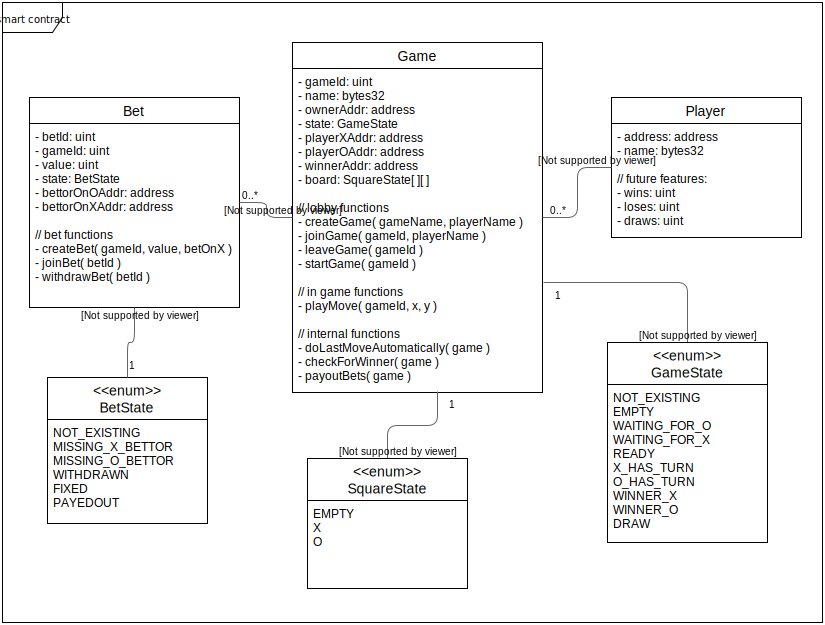
\includegraphics[scale=0.22]{res/sc_uml}
	\end{center}
	\caption{Structure of the \ac{sc}}
	\label{fig:sc_uml}
\end{figure}\newline
\noindent The \ac{sc} can hold multiple games, which always contain one board and two players. Every time a user opens up a new Game, he automatically gets assigned as one of the playing party. Now the Game state is automatically set to 'WAITING\_FOR\_X'. As soon as a second player chooses to enter a open game, the game-owner can start the game, which changes the state to 'X\_HAS\_TURN' as the game has now started and the guest player has to do his first move.\\\\
All Bets contain a game-id pointing to a game which the bet is referencing on it. The user who creates a bet chooses the game and the amount of token he wants to bet with and pays it into the \ac{sc}. Is there an opponent bettor joining the bet, the state changes to 'FIXED'.\\
If the game finds an end, the state of it changes to either 'WINNER\_X', 'WINNER\_O' or 'DRAW', which activates the function 'payout' ,triggering all bets referencing to this particular game. So the bets will change the state to 'PAYOUT' and user will get paid according to their betting.\\ 
Three functions of the \ac{sc} we show here, to discuss in detail the implementation and structure of the \ac{sc}:\\





%logic and modell
